\documentclass{beamer}
\usepackage{graphicx}
\begin{document}
\title{My First Beamer Presentation}
\author{Tim Sizemore}

\begin{frame}
\maketitle
\end{frame}

\begin{frame}
\tableofcontents
\end{frame}

\section{Beamer Basics}
\begin{frame}
\frametitle{Beamer Basics}
\begin{itemize}
\item Use "beamer" as our documentclass rather than "article"
\item We use "fram" to mark the environment for each slide
\end{itemize}
\end{frame}

\section{Images in Beamer}
\begin{frame}
Here's a nice picture:
\begin{figure}[h!]
\begin{center}
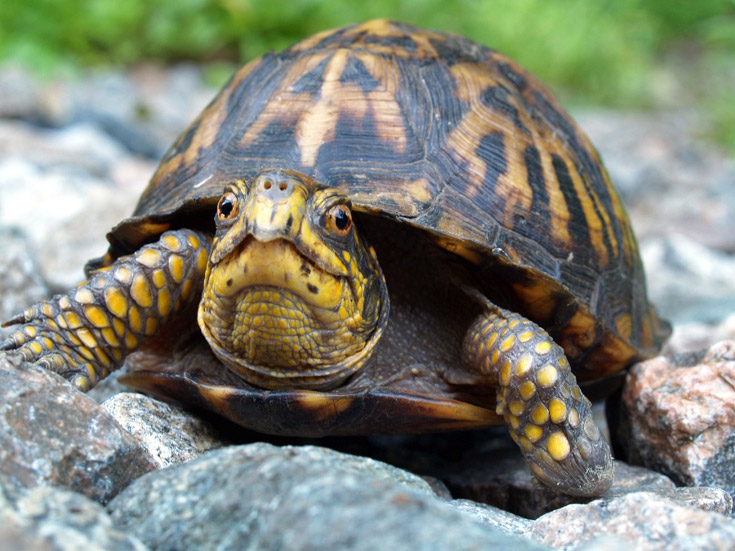
\includegraphics[width=.75\textwidth]{eastern-box-turtle.jpg}
\caption{A turtle, yo!}
\end{center}
\end{figure}
\end{frame}

\section{Switching Views}
\begin{frame}
Showing different items at different steps
\begin{itemize}
\item<1 - > Ineye
\item<2 - > Mineye
\item<3>    Meeny
\item<4>    Mo
\end{itemize}
\end{frame}
\end{document}
